%=== CHAPTER ONE (1) ===
%=== INTRODUCTION ===

\chapter{Introduction}
\begin{spacing}{1.5}
\setlength{\parskip}{0.3in}

The first chapter of the dissertation is almost invariably the Introduction. Generally, its purpose is to lead the readers into the problem you intend to attack in the project, to set the scene. The main points here consist of the background to the problem and your motivation in solving it. This then leads into the objectives and the scope of the project. It is good to conclude your Introduction with a section on the layout of the dissertation. It prepares the readers for what is to come.

\section{Background}

The era of the smart cars is coming, and Advanced-driver-assistance system plays an important role in it. Object detection technologies are used to improve the performance of Advanced-driver-assistance system.

Smart cars equipped with Advanced-driver-assistance system are popular now. With the development of smart driving and Eco-energy technology, more and more companies began to produce and sale the newly designed, electric-driven, smart-driving assistant cars. Leading companies like TESLA, NIO and QuantumScape made hundreds of thousands of cars every year (till 2020)~\cite{petranek2015we}. With these cars bought by more and more families, the smart cars are no longer a concept for common people, but becomes a daily necessities for everyone, as an alternative to a traditional car. Compared with traditional mechanical fuel vehicle, new smart vehicles have many advantages. They are 'new', not only because they are driven by electric energy, but also because they are equipped with intelligent driving assistance systems, which is usually called Advanced-driver-assistance system (ADAS).

\begin{figure}[ht]
\centering
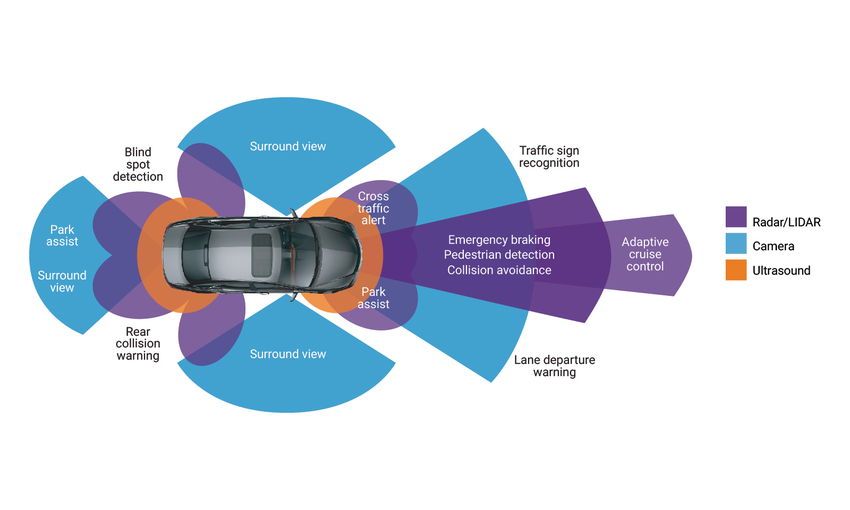
\includegraphics[width=5.5in, fbox]{Chapter1/adas.jpg}
\caption{Advanced-driver-assistance system (ADAS)~\cite{adas}}
\label{fig:adas} 
\end{figure}

ADAS system can reduce road fatalities by minimizing human error. Basic architecture of ADAS system can be shown in \autoref{fig:adas}. Firstly, it utilizes the sensors (LIDAR, in-vehicle camera, GPS) to collect the surrounding obstacle or global position information. Secondly, by combining the information grabbed from all the sensors, the ADAS system can get information that is useful for driving, such as driver's state, current geographical position of cars, the road congestion, potential obstacles on the road, and the trending of road~\cite{morignot2014arbitration}. Such information can be further utilized by the driver or the analysis system to avoid potential dangerous. Because the safety problem is one of the most severe unsolved problems of the traditional human controlled vehicles, ADAS can significantly reduce the death rate related to fatal driving~\cite{brookhuis2001behavioural}.

To improve the performance of ADAS system is an object detection task. ADAS systems use in-vehicle cameras to capture the real-time images of roads~\cite{ziebinski2016survey}. Captured images will be handled by detection module, which recognizes lane outlines and road markings, and then respond to drivers accordingly. This is basically a object detection problem in computer vision area. 

Our work is to solve the problems raised from aforementioned situation, and can be used to improve the performance of ADAS system. 

\section{Motivation}

There are several common issues in aforementioned detection process. 

First is extreme weather and bad illumination conditions. In raining days, images captured by ADAS’s camera may be blurry or be stained by raindrops, and the water on the road may lead to reflection of lights, as shown in figure TBC. In dusk, sun is dim, and the scene is dark-some. The road markings and lane outlines cannot be distinguished from background easily, as shown in figure TBC. With such distortions, the detection algorithm cannot see roads accurately. Consequently, taking measures to denoising is of vital importance. 

Second is curved road. Traditional lane detection algorithms usually work well on straight lane but will meet performance drop once the road turns quickly. One sample of such roads is as in TBC. VPGNet~\cite{lee2017vpgnet} used vanishing point information to solve this problem. Vanishing point is the visual intersection of two parallel lines~\cite{barnard1983interpreting}, here it is treated as the unseen end of the road.  Inspired by the intuition that human eyes utilize the vanishing point to predict the road trending, VPGNet tried to feed this information into neural network by multi-task method. They use multi-task because features employed by VP task, like road curving angle and trending, may also be useful in the detection of lanes and road markings. Based on this, we can expect that with VP information given, the Neural Network can converge better on the other two tasks (lane detection, road marking detection). But VPGNet’s VP feeding scheme is simple, not as efficient as expected. We proposed a new scheme to train with VP information.


Here is a sample of table in \autoref{tabelsample}

\begin{table}[ht]
\centering
\caption{A table without vertical lines.}
\label{tabelsample}
\begin{tabular}[t]{lcc}
\hline
&Treatment A&Treatment B\\
\hline
John Smith&1&2\\
Jane Doe&--&3\\
Mary Johnson&4&5\\
\hline
\end{tabular}
\end{table}%

\section{Motivation}



\section{Objectives and Specifications}



\section{Major contribution of the Dissertation}



\section{Organisation of the Dissertation}


\end{spacing}
%=== END OF CHAPTER ONE ===
\newpage


